\documentclass[11pt]{article}
\usepackage{amsmath}

\usepackage{amstext}

\usepackage{amsthm}
\usepackage{color, fullpage, hyperref}
\usepackage{amssymb}
\usepackage{mathtools}
\usepackage{commath}

\usepackage[table]{xcolor}
\usepackage{makecell}

%\pagecolor[rgb]{0,0,0} %black    % to change page to night mode
%\color[rgb]{0.5,0.5,0.5} %grey

\usepackage{graphicx}
\usepackage{tikz, pgfplots, hf-tikz}
\usetikzlibrary{tikzmark}
\pgfplotsset{compat=1.17}
\allowdisplaybreaks
\renewcommand\qedsymbol{$\blacksquare$}
\usepackage{tcolorbox}
\tcbuselibrary{theorems}
\tcbuselibrary{fitting}
\usepackage{empheq}

\usepackage[margin=0.5in]{geometry}
\usepackage{fancyvrb}

\usepackage{enumerate}
\usepackage{soul}
%\usepackage{alltt}

\usepackage{listings}
\definecolor{codegreen}{rgb}{0,0.6,0}
\definecolor{codegray}{rgb}{0.5,0.5,0.5}
\definecolor{codepurple}{rgb}{0.58,0,0.82}
\definecolor{backcolour}{rgb}{0.95,0.95,0.92}

\definecolor{correct}{RGB}{37,150,190}

%Code listing style named "mystyle"
\lstdefinestyle{mystyle}{
	backgroundcolor=\color{backcolour},   commentstyle=\color{codegreen},
	keywordstyle=\color{magenta},
	numberstyle=\tiny\color{codegray},
	stringstyle=\color{codepurple},
	basicstyle=\ttfamily\footnotesize,
	breakatwhitespace=false,
	breaklines=true,
	captionpos=b,
	keepspaces=true,
	numbers=left,
	numbersep=5pt,
	showspaces=false,
	showstringspaces=false,
	showtabs=false,
	tabsize=2
}

\lstset{style=mystyle}
\tcbset{
	colback=blue!25!purple!10!,
	colframe=blue!40}

\begin{document}
\begin{enumerate}
	\item Miscellaneous short answers.
	\begin{enumerate}
		\item Alan has a file named \Verb|dec25|. He wants to create a link \Verb|xmas| to \Verb|dec25|, such that if \Verb|dec25| is deleted and then a new \Verb|dec25| is created with new content, \Verb|xmas| refers to the new version. Advise Alan on whether the link should be a hard link or symbolic link.
			\begin{tcolorbox}Alan should use a symlink, as a hard link would still point to the original \Verb|dec25| even after it has been deleted and replaced.\end{tcolorbox}

		\item Anne has a file named \Verb|oct31|. She wants to create a link \Verb|hlw| to \Verb|oct31|, such that if \Verb|oct31| is deleted and then a new \Verb|oct31| is created with new content, \Verb|hlw| refers to the old version. Advise Anne on whether the link should be a hard link or symbolic link.
			\begin{tcolorbox}Anne should use a hard link, for the same reason as above.\end{tcolorbox}

		\item Manfred and Natasha are implementing pipelining in C, equivalent to the shell command
			\begin{Verbatim}
prog1 | prog2
			\end{Verbatim}
			Their code fragments are below. What’s wrong in each case? Assume that code not shown but outlined in comments (the “ellided”) is correct.\\
			\begin{tabular}{| c | c |}
				\hline
				Manfred's version & Natasha's version\\
				\hline
				{\begin{minipage}{3in}
						\fvset{tabsize=4}
						\begin{Verbatim}

// pipe creation ellided
pid_t p1, p2;
int s1, s2;
p1 = fork ();
if (p1 == 0) {
	// close and dup2 ellided
	execlp("prog1", "prog1",
	(char*)NULL);
} else if (p1 > 0) {
	// close ellided waitpid(p1, &s1);
	p2 = fork ():
	// rest of code ellided

				\end{Verbatim}
				\end{minipage}} & {\begin{minipage}{3in}
				\fvset{tabsize=4}
				\begin{Verbatim}

// pipe creation ellided
pid_t p1, p2;
int s1, s2;
p2 = fork ();
if (p2 == 0) {
	// close and dup2 ellided
	execlp("prog2", "prog2",
	(char*)NULL);
} else if (p2 > 0) {
	// close ellided waitpid(p2, &s2);
	p1 = fork ();
	// rest of code ellided

			\end{Verbatim}
			\end{minipage}}\\
		\hline
			\end{tabular}
		\begin{tcolorbox}Manfred's \Verb|p2 = fork()| line ends with a \Verb|:| which would cause compiler problems, while Natasha execs \Verb|prog2| before \Verb|prog1|, which is not equivalent to \Verb'prog1 | prog2'\end{tcolorbox}

		\item Tom and Jerry both want their programs to, upon the signal \Verb|SIGINT|, continue normal running and not respond to the signal. Tom sets the signal action to \Verb|SIG_IGN|; Jerry sets the signal action to this no-op handler:\\
		\Verb|void jerry_handler(int sig) { }|

		What happens when Tom’s program calls \Verb|select| and it blocks, and then \Verb|SIGINT| arrives? What happens in Jerry’s case?
		\begin{tcolorbox}In Tom's case, since \Verb|SIGINT| is set to \Verb|SIG_IGN|, the program ignores the signal, while in Jerry's case, since he uses a handler, \Verb|select| will be interrupted and will then return \Verb|-1|.\end{tcolorbox}

		\newpage
		\item In an 8-bit binary number $ b_7b_6b_5b_4b_3b_2b_1b_0 $, we say “bit \#0” for $ b_0 $. E.g., in 00000001, bit \#0 is 1; in 11111110, bit \#0 is 0. Let \Verb|x| be an \Verb|unsigned char| variable. Match the code fragments on the left below to the effects on the right (you may just write the labels “Or”, “Comp”, etc.):\\

		\begin{minipage}[t]{0.3\textwidth}
			\begin{itemize}
				\item[Or.] \Verb'x = x | 1'\tikzmarknode{or}{\Verb|;|}
				\item[Xor.]  \Verb|x = x ^ 1|\tikzmarknode{xor}{\Verb|;|}
				\item[And.] \Verb|x = x & 1|\tikzmarknode{and}{\Verb|;|}
				\item[AndC.] \Verb|x = x & ~1|\tikzmarknode{andc}{\Verb|;|}
			\end{itemize}
		\end{minipage}
		\begin{minipage}[t]{0.6\textwidth}
			\begin{itemize}
				\item[\tikzmarknode{zero}{Zero.}] Change bit \#0 of \Verb|x| to 1; other bits unchanged.
				\item[\tikzmarknode{one}{One.}] Change bit \#0 of \Verb|x| to 0; other bits unchanged.
				\item[\tikzmarknode{comp}{Comp.}] Complement bit \#0 of \Verb|x|, i.e. if 0 change to 1, if 1 change to 0; other bits unchanged.
				\item[\tikzmarknode{else}{Else.}] Something else.
			\end{itemize}
			\begin{tikzpicture}[remember picture, overlay]
				\draw[->, shorten >= 4pt, shorten <= 4pt] (or) to (zero);
				\draw[->, shorten >= 4pt, shorten <= 4pt] (xor) to (comp);
				\draw[->, shorten >= 4pt, shorten <= 4pt] (and) to (else);
				\draw[->, shorten >= 4pt, shorten <= 4pt] (andc) to (one.west);
			\end{tikzpicture}
		\end{minipage}
	\end{enumerate}

\newpage
	\item The Grande Online-Only Cafe wants to give out prizes to a few of its registered customers
	by a lucky draw! They already have a customer file like this:
	\begin{Verbatim}
743 Blanchett Anne anne.b@gmail.com
89 Hathaway Cate meow32@hotmail.com
	\end{Verbatim}

		etc., there are hundreds of more lines. Each line is a customer record with customer ID, family name (restricted to one word), given name (again one word), and email address, using a single space to separate two fields.\\

		Assume that there is a program \Verb|shuf| (actually it exists) that reads lines from stdin and outputs a random permutation of the lines to stdout. Write a shell pipeline that picks 5 random customer lines and outputs them. The output should be alphabetically ordered by family names; if tie, by given names (if still tie, no further tie-breaking necessary).\\

		The complete customer file will come from stdin, and your output should go to stdout. Don’t worry about duplicate customer records.\\

		Note that only a shell pipeline is accepted.
			\lstinputlisting[language=sh]{q2.sh}

	\item Macy’s school computer doesn’t have \Verb|make| installed for some reason! She needs your help writing a shell script that performs a small but important job of \Verb|make|. She has a lot of TeX files (filenames end with “.tex”), and there is a program \Verb|pdflatex| for generating corresponding PDF files. Using “A1.tex” as an example, “\Verb|pdflatex A1.tex|” generates “A1.pdf”. Clearly, she wants to generate if and only if one of:
		\begin{itemize}
			\item A1.tex exists but A.pdf doesn't
			\item both exist, but A1.tex is newer
		\end{itemize}
		“A1.tex” is just an example—this applies to all TeX and PDF files in the current directory.\\ Implement a Bourne shell script to do this.\\
		The command “\Verb|basename A1.tex .tex|” outputs A1 to help you.
			\lstinputlisting[language=sh]{q3.sh}

	\newpage
	\item If you can look up in RAM quickly, you can look up on disk slowly!\\
		In this question, you will write code for binary search tree lookup, but the tree is stored in a binary file on disk! The file consists of 0 or more nodes defined by this struct:
		\fvset{tabsize=4}
		\begin{Verbatim}
typedef struct {
	int key;
	long left, right; // file positions (absolute) or -1L
}   node;
		\end{Verbatim}
		\Verb|key| is a key as usual. Note that instead of pointers to children, we have file positions (offsets) of children, so their types are long as in \Verb|fseek|; accordingly, when there is no left/right child, we use \Verb|-1L| (-1 but type \Verb|long|).\\
		The file may be empty, meaning the tree is empty; but if not, we know that the root node is at the beginning--position 0. Other nodes may be anywhere else, we only know that positions of nodes are non-negative multiples of \Verb|sizeof(node)|.\\

		Implement lookup:\\
		\Verb|int is_present(FILE *f, int needle);|\\
		This looks for \Verb|needle| in the tree in \Verb|f|. It should return 1 (C true) if \Verb|needle| is a key in the tree, 0 (C false) if not.\\

		You do not know where the current file position is before this function begins. You may assume that \Verb|f| allows \Verb|fseek|, and \Verb|fread| on \Verb|f| either hits EOF or succeeds. You may assume that if \Verb|left| is non-negative, the left child node exists at that position; similarly for \Verb|right|.
			\lstinputlisting[language=c]{q4.c}

	\newpage
	\item The files to submit in this question are \Verb|line.h|, \Verb|solve.h|, \Verb|Makefile|\\
		Helen wishes to modularize the following C file into multiple C files for separate compilation.
		\begin{Verbatim}
#include <stdio.h>
typedef struct {
	double m, c; // as in y=mx+c
} line;

double compute_y(const line *L, double x) {
	return L->m * x + L->c;
}

typedef struct {
	double x, y;
} point;

int solve(point *p, const line *L1, const line *L2)
{
	double d = - L1->m + L2->m; if (d == 0) return 0;
	else {
		p->x = L1->c - L2->c;
		p->y = - L1->m * L2->c + L2->m * L1->c; return 1;
	}
}

int main(void)
{
	line L1, L2;
	point P;
	L1.m = 4;
	L2.m = -2; L2.c = 2; printf("%f\n", compute_y(&L1, 0)); solve(&P, &L1, &L2);
	printf("%f %f\n", P.x, P.y);
	return 0;
}
		\end{Verbatim}
	\newpage
		\lstinputlisting[language=c, title=\Verb|line.h|]{line.h}
		\lstinputlisting[language=c, title=\Verb|solve.h|]{solve.h}
		\lstinputlisting[language=make, title=\Verb|Makefile|]{Makefile}

	\newpage
	\item In this question, you will implement in Q6.c (starter provided) setting up the processes and pipes in this diagram (there is also a parent process lurking, not shown):\\[-5pt]
		\begin{center}
			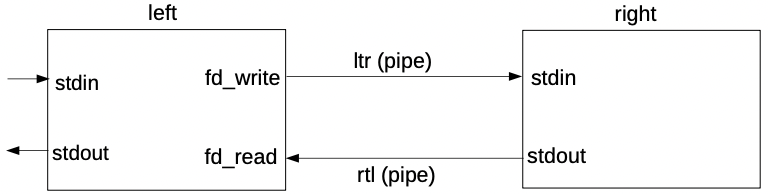
\includegraphics[scale=0.8]{q6.png}
		\end{center}
		The right process will eventually exec a program that isn’t aware of this setup except to read from stdin and write to stdout. Therefore before exec, you will set up stdin to be the read end of the ltr pipe, stdout to be the write end of the rtl pipe.

		The left process won't exec, instead call

		\Verb|void do_left(int fd_read, int fd_write);|

		Therefore you will call \Verb|do_left| so that \Verb|fd_read| is the read end of the rtl pipe, \Verb|fd_write| is the write end of the ltr pipe. Note that the left process inherits stdin and stdout from the parent, and \Verb|do_left| can perform I/O on all 4 distinct FDs.\\
		Both left and right are child processes of a common parent. The code is structured as follows:
		\begin{Verbatim}
void leftright(void)
{
	// parent begins
	int ltr[2];
	int rtl[2];

	pipe(ltr);
	pipe(rtl);

	pid_t left = fork();
	if (left == 0) {
		// left child code , part (a)
	} else {
		pid_t right = fork();
		if (right == 0) {
			// right child code , part (b)
			execlp("right", "right", (char*)NULL);
			exit(1);
		} else {
			// parent code after both forks, part (c)
			wait(NULL);
			wait(NULL);
		}
	}
}
		\end{Verbatim}
			\newpage
			\begin{enumerate}
				\item Complete the code for the left child.
					\lstinputlisting[language=c]{left6.c}
				\item Complete the code for the right child.
					\lstinputlisting[language=c]{right6.c}
				\item Complete the code for the parent after forking and before waiting.
					\lstinputlisting[language=c]{main6.c}
			\end{enumerate}

	\newpage
	\item The \Verb|do_left| from the last question\\
	\Verb|void do_left(int fd_read, int fd_write);|

	actually does this job:
		\begin{itemize}
			\item Copy data from \Verb|fd_read| to stdout, verbatim.
			\item Copy data from stdin to \Verb|fd_write| \textbf{but} change all lower case letters to upper case (in the sense of \Verb|toupper|).
		\end{itemize}
		Since there are two data sources with unknown arrival times, \Verb|select| is a simple way to wait for data, given that the two input FDs won’t change.

		Implement \Verb|do_left|. Use buffer sizes of 512 bytes. You may assume that \Verb|write| is successful and doesn’t block. You may assume \Verb|fd_read| $ \ne $ 0. When any of the input sources gives EOF, call \Verb|exit(0)|.
			\lstinputlisting[language=c]{q7.c}
\end{enumerate}
\end{document}